\documentclass[conference]{IEEEtran}
\IEEEoverridecommandlockouts
% The preceding line is only needed to identify funding in the first footnote. If that is unneeded, please comment it out.
\usepackage{cite}
\usepackage{amsmath,amssymb,amsfonts}
\usepackage{algorithmic}
\usepackage{graphicx}
\usepackage{float}
\usepackage{textcomp}
\usepackage{multirow}
\usepackage{amsmath}
\usepackage{xcolor}
\def\BibTeX{{\rm B\kern-.05em{\sc i\kern-.025em b}\kern-.08em
    T\kern-.1667em\lower.7ex\hbox{E}\kern-.125emX}}
\begin{document}



%% PUT YOUR PROJECT TITLE HERE
\title{Classifying Maternal Health Risk With Various Feature Selection Algorithms
}

\author{

\IEEEauthorblockN{Yagya Malik}
\IEEEauthorblockA{
\textit{CIS6930}\\
Gainesville, FL, USA \\
yagyamalik@ufl.edu}
\and
\IEEEauthorblockN{Abhiti Sachdeva}
\IEEEauthorblockA{
\textit{CIS6930}\\
Gainesville, FL, USA \\
abhitisachdeva@ufl.edu}
\and
\IEEEauthorblockN{Akshat Shrivastava, Daanish Goyal }
\IEEEauthorblockA{
\textit{CIS6930,CIS6930}\\
Gainesville, FL, USA \\
a.shrivastava@ufl.edu, dg5052@gmail.com}
}

\maketitle

\begin{abstract}
Maternal health refers to the mannerism adopted
toward women's health and well-being during a prenatal and
postnatal phase. It comprehends the women's physical, mental, emotional, and social well-being from antenatal to
delivery aftercare. This research envisions the technological advancement in AI and mobile sensors as a new framework. With the widespread adoption of smartphones and the internet, the use of low cost and accessible sensors can allow
the collection of health vitals irrespective of the availability of massive
infrastructure, healthcare professionals, and high-end medical gad-
gets. The data analysis, machine learning classification techniques, and feature selection algorithms described in this paper can be
used with data from sensors to classify risk into three categories
(high risk, low risk, medium risk). The methodology described
in this project has achieved 87.49\% accuracy using three health
data points, derived using Information Gain feature selection
and Random Forest classification model. This critical information
helps provide quality emergency obstetric care and
is expected to avert many antenatal and postnatal
complications. The timely intervention may accelerate the routine
health checkup system sequentially, helping the attainment of
the Millennium Development Goal for maternal health. The research
aims to provide testable solutions for universal maternal
care and enlightenment governed by central tenets of equity for
skilled health mediation and dignified and respectable maternal care
globally.
\end{abstract}

\begin{IEEEkeywords}
Health Data, Data Science, Feature Selection
\end{IEEEkeywords}

\section{Introduction}

Maternity, or motherhood, is the period during pregnancy and shortly after childbirth. A woman's overall health and well-being during pregnancy, childbirth, and post-natal period is referred to as maternal health. Maintaining maternal health usually involves taking care of factors that can directly or indirectly affect the mother or her child's health. The number of women who face various challenges during childbirth every year is concerning. The severity of the complications could even result in the loss of life. In 2015, around
300,000 women died due to complications during childbirth, as reported by WHO \cite{TMM}. Approximately 86\% of the global maternal deaths were from Sub-Saharan Africa and Southern Asia, with Sub-Saharan Africa contributing roughly two-thirds to the estimated total \cite{whoMM}. 

Data from a UNFPA report claims that socio-economic factors like inadequate access to healthcare and poverty contribute to an increase in the risk of maternal mortality \cite{unfpareport}. The
lack of a proper health care system and, more importantly, the infrastructure required for the proper care of pregnant women
especially in third world countries could be attributed to this.
This leads to worrying figures like the ones we discussed
above.
Several efforts have been made to overcome this challenge,
such as EPMM strategies developed by WHO \cite{eemstrat} and the HHS initiative \cite{hhsinit} and have shown some improvements. For
the period 2000 to 2010, Southern Asia showed the most improvement and had the most significant overall reduction in Maternal Mortality Ratio (MMR). However, the situation does not seem to get better with recent data showing that about 808 women lose their lives every day due to a preventable cause relating to pregnancy \cite{unfpamathlth}.

With the recent advancements in technology, we have highly capable medical devices and sensors capable of measuring important health vitals on the fly. In addition to this, the widespread use of smartphones that are embedded with these sensors have enabled the development of sophisticated machine learning algorithms that could help detect and monitor these conditions without the need for regular in-person visits, checkups, and expensive screening tests. With this project, we aim to select the most relevant health data points that influence maternal health using feature selection, and then test several machine learning classification models for predicting maternal health risk by analyzing their accuracy.
This paper is structured in the following way: In Section 2, we explain our motivations behind this project and provide insights into the landscape of maternal healthcare for women. Section 3 includes information about the data set we used for our analysis and a brief introduction to the features and their respective domains. In Section 4, we give a thorough explanation of data pre-processing steps taken, the various feature selection techniques used, and the machine learning models we used to test our selected features. These are followed by the
results of our analysis in Section 5. In Section 6, we briefly discuss our findings and their implications. Section 7 details related studies in this area, and in Section 8, we conclude by giving some final thoughts and discussing future work in this space.

\section{Motivations}
The WHO and MoHFW endorse fundamental access to respectful and continuum maternity care. The attitude, knowledge and the lack of resources are critical factors associated with maternal health's high morbidity and mortality rate. The SDGs or Global Goals strive to bring the maternal mortality ratio down to 0.7\% by 2030. This ambitious target is an essential human rights imperative, and the best way
to ensure its implementation is coverage to the third world
countries at the grass-root level.

In addition to this, one of the main challenges that developing nations face today is inadequate access to quality
healthcare. The number of healthcare professionals per 10,000
people are only 11 in Africa \cite{anand2004human}. This number is astonishing compared to Europe, which has 79 healthcare professionals per 100 people. According to a WHO report, a number less than 23 for a nation would not be enough to meet the essential requirements for target MDG \cite{worldhealthstat}.

Another exciting report by WHO claims that the technologies required for preventing maternal morbidities and mortalities already exist, and this is one of the reasons why maternal deaths are labeled as ``avoidable" or ``preventable." \cite{whoreduce}. Additionally, they also state that interventions for improving maternal health and reducing mortality rates could be cost-effective \cite{whomathlth}. With our research, we aim to develop and test a model that could prove to be useful in the development of such cost-effective interventions.

\section{Case of study}
The Maternal Health Risk data set is a public data set collected from the UCI Machine Learning Repository. Thevdata in this database has been collected via various sources, such as public hospitals, community clinics, and maternal health cases from rural areas in Bangladesh. This was done using an IoT-based risk monitoring system. The data set consists of 1014 instances with nine numerical attributes and a multi-class decision attribute with no missing values.
We describe the attributes in the table below:

\begin{table}[!h]
\begin{tabular}{lll}
No of features     & Name of features         & Min/max \\
\multirow{8}{*}{9} & \multicolumn{1}{l}
                    {Age (Years)} &         Numerical value in range 10-70\\
                   & Weight (Kg)              &    Numerical value in range 45.5-90.3     \\
                   & SystolicBP              &     Numerical value in range 70-160    \\
                   & DiastolicBP              &     Numerical value in range 49-100    \\
                    & Blood Sugar (mmol/L)              &     Numerical value in range 6-19    \\
                   & HeartRate  (bpm)              &   Numerical value in range 7-90     \\
                   & Blood\_oxygen\_level     &     Numerical value in range 90-99    \\
                   & BodyTemp\_F              &      Numerical value in range 98-103   \\
                   & BodyTemp\_C              &      Numerical value in range 36.7-39.4  
\end{tabular}
\end{table}
% Please add the following required packages to your document preamble:
% \usepackage{multirow}


The multi-class decision attribute is described below -
\begin{itemize}
    \item RiskLevel (HighRisk, MedRisk, LowRisk)
\end{itemize}
\section{Proposal of solution}

The primary purpose of our project is to predict and evaluate maternal health risks efficiently and accurately using several machine-learning feature selection and classification algorithms. We also present and compare results with and without feature selection applied to different classifiers to measure which set of features and classifier gives the most accurate result for predicting maternal health risks. We implement the classifiers on our selected data set and test it using accuracy scores.

Feature selection algorithms were implemented to reduce the number of attributes from our data set. This was done to identify the optimal set of attributes that could used for monitoring maternal health.
Below we detail the various steps we followed and a flowchart of the proposed work is presented in figure \ref{fig:proposal}.
\begin{figure}[!h]
    \centering
    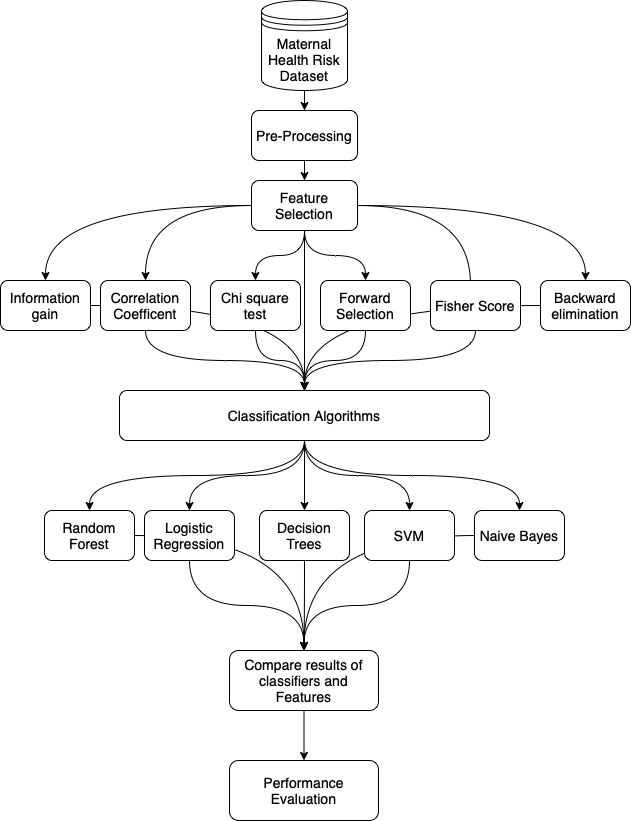
\includegraphics[width=\columnwidth]{Diagram.drawio.jpeg}
    \caption{Our proposed methodology }
    \label{fig:proposal}
\end{figure}
\begin{enumerate}
    \item \textbf{Database selection: } The maternal health risk data set was uploaded to the UCI website in CSV file format. We imported this data to a python notebook and converted it into a pandas data frame for further processing.
    \item \textbf{Pre-processing and transforming data:} The data was scanned for any constant features, quasi-constant features, missing records, and duplicated records. Furthermore, categorical features were labeled with numerical values to apply classification algorithms.
    \item \textbf{Feature selection:} Since the data in the data set was collected from a public database, a plethora of attributes were collected from the patients, but only a few of they ought to be relevant for classifying maternal risk. To remove such noisy and redundant information, we implore the use of feature selection techniques. The different feature selection techniques we used for our problem was Correlation Coefficient, Information Gain, Chi-square test, Fisher score, Forward selection and Backward Elimination.
    \begin{enumerate}
        \item \textbf{Correlation Coefficient:} It is a measure that determines the degree to which two variables are associated with each other \cite{corrcoeff}. We employed this technique to potentially remove attributes that have a linearly dependency and reduce redundancy in our data.
        \item \textbf{Information Gain: } Information gain is defined as ``measure of how much information a feature provides about a class." \cite{infogain}. We employed the use of information gain so it could tell us how sound each of the features is in discriminating between classes (high risk, medium risk, low risk) by calculating entropy.
        \item \textbf{Chi-squared Test: } Chi square test is used to measure how an Observed count (O) deviates from and Expected count (E) \cite{chi2}. This technique is used to determine independent features (which have no association between them) that highly impact the classification (high risk, low risk, medium risk) by comparing the chi-square value between them.
        \item \textbf{Fisher Score: } Fisher score evaluates the rank of each of the attributes in determining risk based on maximum-likelihood equations (fisher score). This would allow us to select features based on their fisher score ranks.
        \item \textbf{Forward feature selection: } For this iterative technique, we begin with an empty set of attributes and keep adding to it features that result in an increase in performance till no further improvement can be achieved.
        \item \textbf{Backward Elimination: } Similar to Forward Selection, in this iterative technique, we begin with a complete set of attributes and eliminate the least significant attributes based on performance in each iteration. This is repeated until no further improvement is achieved on removing attributes.
    \end{enumerate}
    \item \textbf{Classification: }We use machine learning algorithms to predict states of maternal health risk (low, medium, or high). The following classifiers were implemented on the features selected by the previous step.
    \begin{enumerate}
        \item \textbf{Naive Bayes:} This algorithm is based on Bayes' Theorem \cite{bayestheorem} and works on the assumption that the presence of a particular attribute is unrelated the presence of any other attribute. 
        \item \textbf{Support Vector Machines (SVM): } SVM is a supervised learning model that calculates a hyperplane in an N-dimensional plane (N being the number of features) that best classifies the data points \cite{svm}.
        \item \textbf{Logistic Regression: } Although it is used to predict continuous target variables, It is a powerful tool for solving classification problems \cite{logreg}. The core of Logistic Regression is its logistic function, also called the sigmoid function. It takes real numbers as input and outputs a value between 0 and 1. 
        \item \textbf{Decision Trees: } Are used for imitating decision-making processes with the help of leaves and branches. Each branch represents a decision or a rule, and each leaf node is equivalent to an outcome.  
        \item \textbf{Random Forest: } It combines the outputs of multiple decision trees to deduce a single result. This algorithm is used for both classification and regression problems.
        
    \end{enumerate}
    \item \textbf{Performance evaluation: }To determine the least and a most accurate set of features and the best classification an algorithm, performance from each classifier (over different features) is evaluated using an accuracy score. The accuracy score can be described by the formula: \\
    \begin{equation}
\text { Accuracy }=[\dfrac{(\mathrm{TP}+\mathrm{TN}) }{(\mathrm{TP}+\mathrm{FP}+\mathrm{FN}+\mathrm{TN})}]
\end{equation}
Where TP stands for True Positives, TN stands for True Negatives, FP stands for False Positives, FN stands for False Negatives.
\end{enumerate}

\section{Results}

\textbf{Feature selection with correlation coefficient:}
 A value close to 1 implies a strong positive correlation on the other hand, a value close to -1 implies a strong negative correlation and 0 implies no correlation. The resulting correlation matrix is illustrated in Fig \ref{fig:corrmatrix}
\begin{figure}[!h]
    \centering
    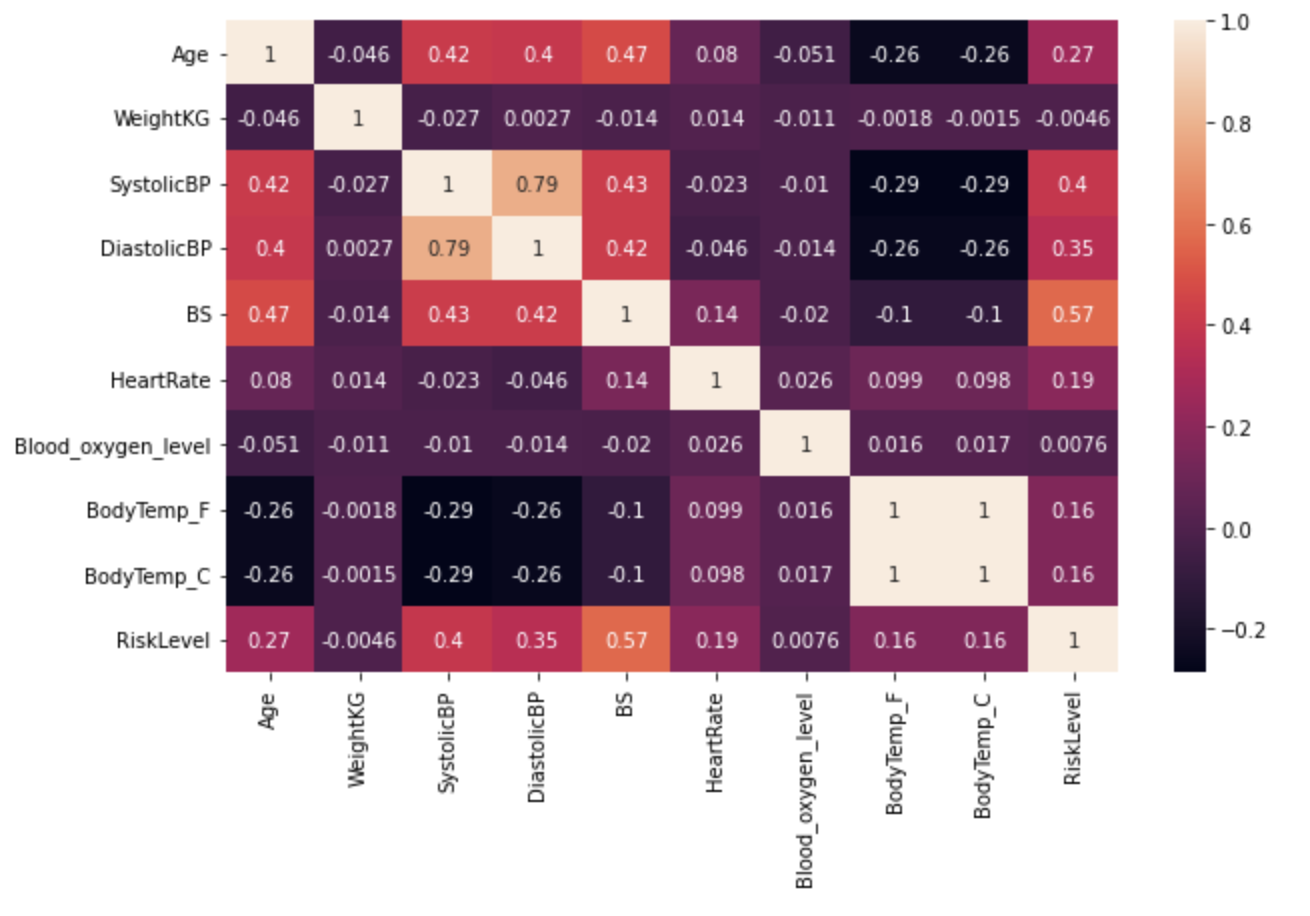
\includegraphics[width=\columnwidth]{Screen Shot 2022-04-15 at 1.28.37 PM.png}
    \caption{Correlation matrix achieved for the set of attributes in our data set}
    \label{fig:corrmatrix}
\end{figure}
\\ The correlation between BodyTemp\_F and BodyTemp\_C is noted here.
\\
\textbf{Feature selection with Information gain:}
Figure \ref{fig:iggraph} depicts information gain of each of the attributes in context to the target variable (risk level). The top 3 features from this algorithm were chosen for further classification. \\
\begin{figure}[!h]
    \centering
    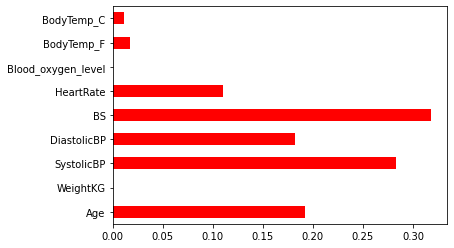
\includegraphics[width=\columnwidth]{Information_gain.png}
    \caption{Information gain graph generated for the set of attributes in our dataset}
    \label{fig:iggraph}
\end{figure}
\\
The selected features from above mention algorithms, along with results from all the other feature selection algorithms that we applied can be found in Figure \ref{fig:Featureresult}
\begin{figure}[!h]
    \centering
    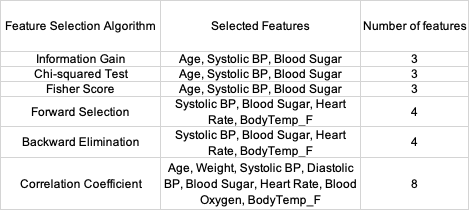
\includegraphics[width=\columnwidth]{IMG_8566.png}
    \caption{Results of feature selection algorithms}
    \label{fig:Featureresult}
\end{figure}
\\
For accurately judging the benefits of using different feature selection techniques, we performed some initial tests on the original data set with the following classification algorithms:
\begin{itemize}
    \item Random Forest
    \item Logistic Regression
    \item Decision Tree
    \item Support Vector Machines
    \item Naive Bayes
\end{itemize}

The accuracy scores achieved have been listed in Figure \ref{fig:orig}

\begin{figure}[!h]
    \centering
    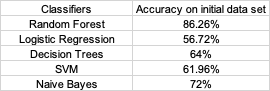
\includegraphics[width=5cm]{IMG_9611.png}
    \caption{Performance of different classification algorithms for the original data set}
    \label{fig:orig}
\end{figure}

\\To determine the most favourable set of features and the best classification algorithm, we evaluate the performance of each classifier against each feature set. The results of these tests have been listed in Figure \ref{fig:classification1}

\begin{figure}[!h]
    \centering
    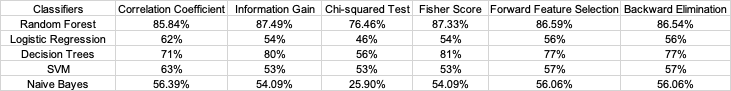
\includegraphics[width=\columnwidth]{IMG_3789.png}
    \caption{Performance of different classification algorithms with feature selection }
    \label{fig:classification1}
\end{figure}
\\
We visualised these results and present a graphical interpretation of the same against the original data set in Figure \ref{fig:classification2}
\begin{figure}[!h]
    \centering
    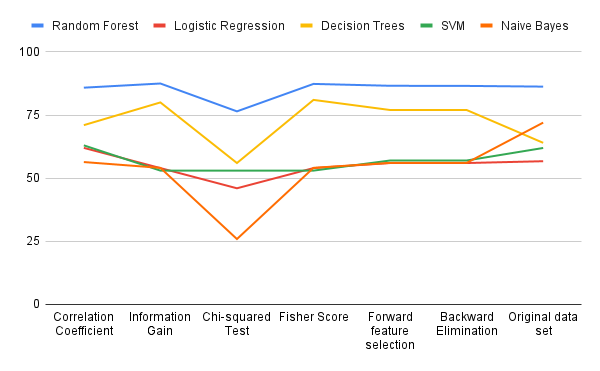
\includegraphics[width = \columnwidth]{chart (1).png}
    \caption{Performance of different classification algorithms with feature selection }
    \label{fig:classification2}
\end{figure}
\\
\section{Discussion}

The data collected from the UCI database consists of health data attributes that were recorded using several sensors equipped within an IoMT device. 
Using the methodology we described in this paper, it is possible to reduce the number of health attributes that are necessary to classify maternal health risk level and increase accuracy at the same time. 

We noticed an overall increase in the accuracy of classifications by employing feature selection techniques. Almost all of the classifiers showed an increased performance. This can be observed in Figure \ref{fig:withvswithout}. We have also indicated the number of features in both the sets. 
\begin{figure}[!htp]
    \centering
    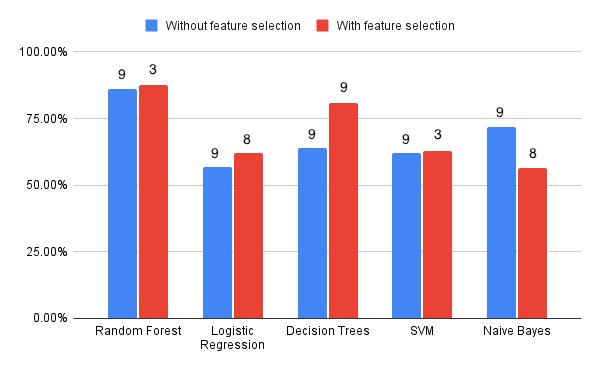
\includegraphics[width = \columnwidth]{chart(2).png}
    \caption{ Performance of classifiers with and without feature selection }
    \label{fig:withvswithout}
\end{figure}
\\
Our analysis achieved the highest accuracy of 87.49\% using only 3 features out of the total 9 with the help of Random Forest classifier and features selected using Information Gain. 

Performing feature selection with Information Gain tells us that Age, Systolic Blood Pressure and Blood Sugar are the primary determinants of Maternal Health risks. These vitals can be measured using only 2 sensors compared to the 7 sensors that the IoMT device was embedded with. 

Since predicting maternal health risk is a real-world problem, we believe that such optimization would not only increase the feasibility of such technologies in being a part of health care systems but would also reduce the costs associated with devices that allow digital monitoring of health data significantly.

\\
\section{Related Work}
In 2007, Huang et al. \cite{huang2007feature} did a study where they applied feature selection techniques similar to the ones described in our study on a data set consisting of diabetic patient's health information. They aimed to select the most influential feature in determining diabetes. They also used several machine learning classification algorithms to classify patient's data. They reported an accuracy of 95\% using a reduced set of features.

A similar study was done by Selvakuberan et al. \cite{selvakuberan2011efficient} where they combined several datasets collected from PIMA Indian Diabetes Dataset. This study was much more extensive than the study done by Huang et al. as they used a much broader combination of data sets. With their feature selection techniques, they were able to increase accuracy by 16\%, from 65\% the highest accuracy without feature selection and 81\% accuracy with feature selection.


Ramesh et al. \cite{ramesh2021improving} did a study in 2021 intending to test the accuracy of machine learning models in the early prediction of heart-rate diseases. They implored the use of Information Gain \cite{infogain} feature selection algorithm along with SVM \cite{svm} classification model for prediction. They reported highest prediction accuracy of 88\% with a reduced set of features.


With a similar interest, in 2020 Spencer et al. \cite{spencer2020exploring} did a study where they used a combination of feature selection and classification models compared to just one applied by Ramesh et al. reported the highest accuracy of 85\%. In their study, Spencer et al. also provided several other performance criteria to measure their classification models, such as recall and precision. These performance metrics can be implemented in future studies for a better understanding of the performance of the classification and feature selection models

\section{Conclusions and Future Research Lines}
Machine learning and Digital Health technologies are at the forefront of the worldwide battle against increasing maternal mortality rates. With this research, we planned to investigate the feasibility and performance of classification and feature selection models available to us. Our work shows that
classifying maternal health risks using medical IoT devices is possible through the use of Machine Learning. Furthermore, the accuracy of such classification algorithms depends highly on the feature selection technique used. We could achieve the highest accuracy of 87.49\% using Information Gain feature selection with Random Forest Classifier. Another result of note that had similar accuracy was using Fisher Score feature selection with Random Forest classification. Such
lightweight machine learning algorithms and cost-effective sensors required to collect these essential health data points could be used to effectively screen maternal health risks followed by a more in-depth routine checkup.

After analyzing the results from the various feature selection algorithms applied by us, it is clear that Systolic Blood Pressure is the most influential feature for predicting maternal health risk, followed closely by Blood Sugar and Age. Even though these features are ranked differently across the different
feature selection algorithms we used, they still give us the most accurate prediction.

Our work is limited in its scope because we have only applied a small selection of classifiers and feature selection algorithms available. By applying more advanced algorithms, it would be possible to develop an even more accurate classification algorithm. Extensive experimentation and analysis using different machine learning algorithms and feature selection algorithms that are tailored toward the data set could be beneficial in the development of such models. The method that we proposed in this study could be adopted by hospitals or healthcare professionals to monitor patients with minimal use of sensors or costly medical equipment. The features selected by our processing are also significant for future research and development in this space.

\bibliographystyle{IEEEtran}
\bibliography{mybib.bib}

\end{document}
